\documentclass{article}

\title{The plan-execute pattern}
\subtitle{A ubiquitous pattern you won't find in your textbook.}
\date{2024-06-20}
\modified{2024-06-20}
\keyword{programming}
\keyword{software-design}

\begin{document}
\section*

I feel uneasy about design patterns.
On the one hand, my university class on design patterns revived my interest in programming.
On the other hand, I find most patterns in the \href{https://www.goodreads.com/book/show/85009.Design_Patterns}{Gang of Four} book to be irrelevant to my daily work;
they solve problems that a choice of programming language or paradigm creates.

My litmus test of a good design pattern is its cross-disciplinary applicability.
I'm more likely to accept an idea that pops up in fields beyond software engineering.
And the most convincing patterns are the ones that help me in everyday life.

This article describes a universal pattern that billions of people rely on daily, but software engineers rarely discuss---the plan-execute pattern.

\section{background}{Background}

In early August 2020 I was working on \textsc{dfinity}'s \href{/posts/02-ic-state-machine-replication.html#incremental-sync}{incremental state synchronization protocol}.
The protocol brings a stale replica up to date by computing and applying state deltas on top of an existing state snapshot.

One major challenge with this protocol was testing.
If the protocol implementation is a black box that outputs the final state, then how do I check that it took the most efficient path to reconstruct the checkpoint?
Simply observing the output won't work: it might have decided to fetch the entire new state instead of re-using locally available pieces.

To address this problem, I factored the implementation into stages:
\begin{enumerate}
  \item Acquire all the information required for synchronization: the bill of materials for the local and target replica states.
  \item Build a \emph{plan}---a data structure encapsulating the protocol decisions: what data to fetch, what to copy from the local state, and how to assemble the pieces.
  \item Execute: fetch the data and schedule disk writes according to the plan.
\end{enumerate}

Since then, the pattern has become one of my favorite techniques.
I used it a few more times with great success and started recognizing it in other software.

\section{plan}{Plan}

\epigraph{
    Planning can be seen as reformulating a problem in a simpler problem space, solving it in the simpler space, and then trying to generalize that approach to the real problem space.
}{Scott H. Young, ``Get Better at Anything''}

There are two ways to get from Washington, \textsc{dc}, to New York City by car.
One approach is getting in your vehicle, starting the engine, and following the road signs until you reach the destination.
I call this approach ``just do it.''
Alternatively, you can sit down with a map and plan your itinerary, deciding which routes you will take and where you'll stop for a break, and then follow the planned route.
That's the plan-execute approach.

In software engineering, we often deal with complex algorithms that can take many paths to reach their goals.
A ``just do it'' implementation freely interleaves decisions and actions, hiding the execution details from observers.

\begin{figure}[grayscale-diagram]
\marginnote{mn-just-do-it}{
  The ``just do it'' implementation of an algorithm hides all decisions it takes.
}
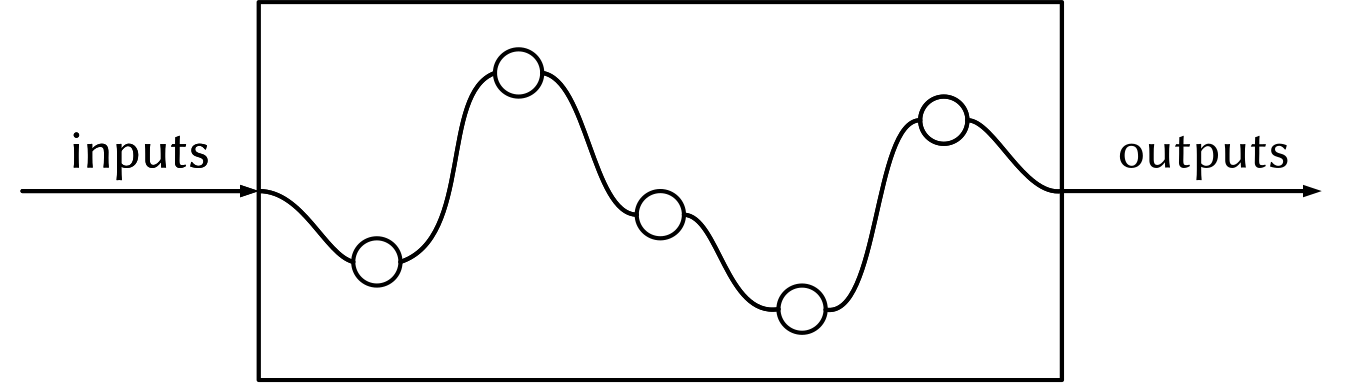
\includegraphics{images/29-just-do-it.svg}
\end{figure}

The plan-execute pattern tackles the problem in two stages.
The planning stage takes the inputs and produces a plan: a data structure encapsulating all the decisions the algorithm should make.
The execution stage realizes the plan.

\begin{figure}[grayscale-diagram]
\marginnote{mn-plan-execute}{
  The plan-execute pattern consists of two stages: the planning stage outputs the decisions as a data structure, and the execution stage realizes the plan.
}
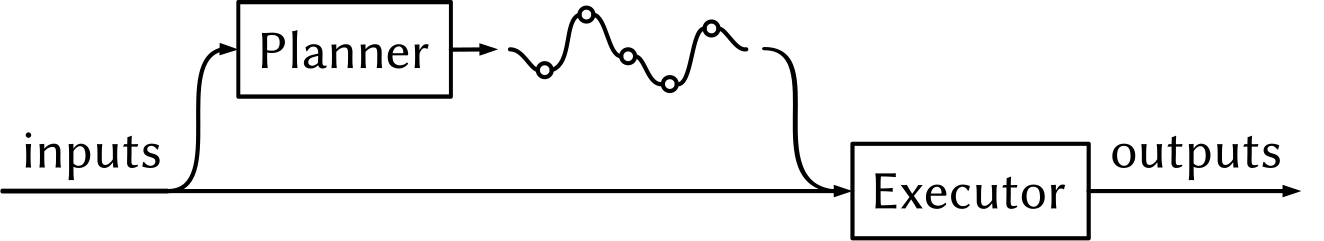
\includegraphics{images/29-plan-execute.svg}
\end{figure}

This approach allows for more comprehensive testing of the decision-making part.
It also extends the system's debugging capabilities: since the plan is a data structure, humans can inspect it to understand what the system is about to do without causing \href{https://en.wikipedia.org/wiki/Side_effect_(computer_science)}{side effects}.

\section{execution}{Execution}

\epigraph{If you want to make God laugh, tell him about your plans.}{Woody Allen}

In some cases, the execution part of the pattern is straightforward: traverse the plan data structure and run predefined steps:
Turn left, turn right, \href{https://xkcd.com/461/}{take the ferry across the lake}.
That works well if the execution environment is predictable.

When driving a car, however, we might have to take an unplanned route because of traffic, weather conditions, missed turns, and construction work.
Similarly, when execution steps can involve concurrency or potential failure, our programs must adjust the plan as they realize it.

My favorite way to deal with uncertainty is to split the execution stage further into a state machine and a driver loop.
The driver feeds external events into the state machine, and the state machine emits actions that the driver must take.
The original plan becomes an initializer for the state machine starting state.

\begin{figure}[grayscale-diagram]
\marginnote{mn-dynamic-planning}{

}
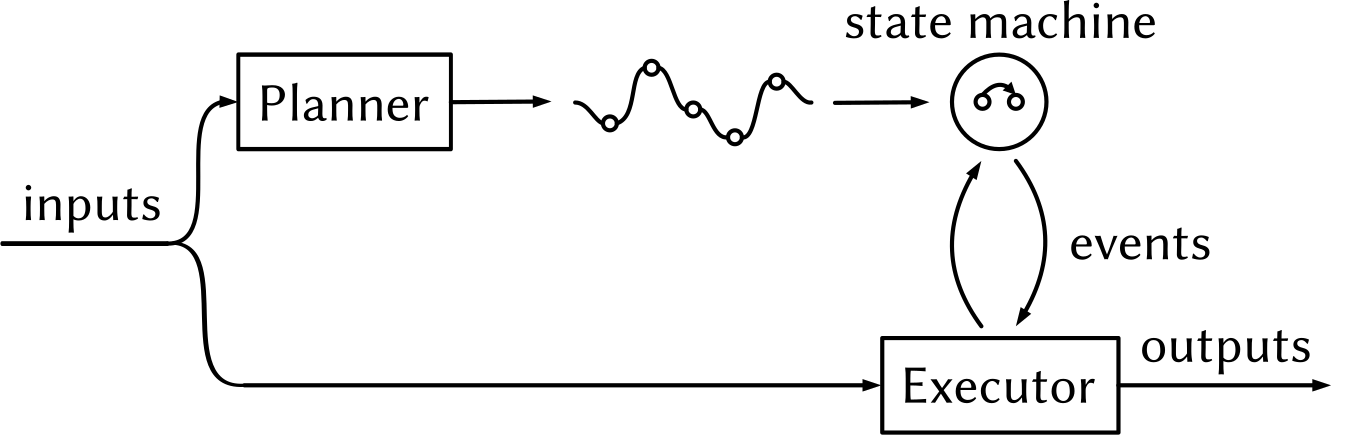
\includegraphics{images/29-dynamic-planning.svg}
\end{figure}

The beauty of this approach is that the state machine doesn't depend on messy execution details,
so we can test it exhaustively and thoroughly,
potentially applying \href{https://propertesting.com/book_state_machine_properties.html}{property-based testing techniques}.

\section{build-system-example}{Build system example}

The following simplistic build system design demonstrates how all the pattern pieces fit together.
The inputs for a build are the build graph, the set of outputs the caller requested to materialize, and the build cache state.
The plan is the list of tasks we need to execute to materialize the desired artifacts, in the topological order.

\begin{code}[rust]
struct Node {
    id: NodeId,
    inputs: Vec<ArtifactId>,
    outputs: Vec<ArtifactId>,
    transform: Command,
}

struct BuildGraph(\ldots)

type BuildPlan = Vec<Node>;

fn plan(
    g: &BuildGraph,
    cache: &BuildCache,
    targets: &[ArtifactId],
) -> Result<BuildPlan, BuildError> { \ldots  }
\end{code}

The most straightforward execution function would go over the tasks in the plan and execute them sequentially.

\begin{code}[rust]
fn run_build_sequentially(
    plan: &BuildPlan,
    cache: &BuildCache,
    sandbox: &Sandbox,
) -> Result<(), BuildError> {
    for node in plan {
        sandbox.execute(node, cache)?;
    }
    Ok(())
}
\end{code}

A more efficient approach is to implement pipeline parallelism and execute independent tasks concurrently.
This execution model adds a lot of complexity, which the build plan alone doesn't address.
So we introduce a state machine that keeps track of unfinished work and adjusts the plan as the execution unfolds.

\begin{code}[rust]
struct ExecutionState {
    graph: BuildGraph,
    todo: Vec<NodeId>,
    in_progress: Vec<NodeId>,
    depcount: HashMap<NodeId, usize>,
}

enum Action {
    Schedule(Vec<Node>),
    Finish,
}

impl ExecutionState {
    \emph{// Returns the first action to take.}
    fn init(&self) -> Action { \ldots  }

    \emph{// Indicates that the task corresponding to the node is in progress.}
    fn started(&must self, node: NodeId) { \ldots  }

    \emph{// Indicates that the task corresponding to the node has been completed.}
    \emph{// Returns the next action to take.}
    fn completed(&mut self, node: NodeId) -> Action { \ldots  }
}
\end{code}

The \code{run\_build} function is the driver loop that spawns processes and feeds their results to the state machine, which either outputs more tasks or reports that the build has finished.

\begin{code}[rust]
fn run_build(
    cache: &BuildCache,
    sandbox: &Sandbox,
    state: ExecutionState,
) -> Result<(), BuildError> { \ldots  }
\end{code}

This design splits a hard problem into smaller pieces that are easy to understand.
The most algorithm-heavy portions (planning and execution control) do not require any I/O and are easy to test.
Only the \code{run\_build} function needs to interact with the operating system.
The planning function is also helpful in implementing the \code{--dry-run} feature.

\section{instances-relatives}{Instances and relatives}

The \href{https://en.wikipedia.org/wiki/Query_plan}{\textsc{rdbms} query planner} is a supreme example of the pattern.
There are many ways to execute an \textsc{sql} query, and the database engine should always use the most efficient one.
Query plans give us insight into which path the engine is going to take; they are paramount for understanding and tweaking database performance.

The \href{https://en.wikipedia.org/wiki/Interpreter_pattern}{interpreter pattern} is a special case of the plan-execute pattern,
where plans are syntactic trees expressing the intent,
and the execution stage is their interpretation.

The \href{https://sans-io.readthedocs.io/how-to-sans-io.html}{Sans-\textsc{i/o}} protocol implementations provide a blueprint for extracting execution state machines from input/output driver loops
as discussed in the \href{#execution}{Execution} section.
This practice goes back to functional programming folklore;
\href{https://www.destroyallsoftware.com/talks/boundaries}{Gary Bernhardt} called it ``functional core, imperative shell''.

Finally, all programs are plans: a programmer makes all decisions in advance and encodes them as a byte array,
leaving it to the computer to take care of the execution.
``Programming'' was a synonym of ``planning'' before computers conquered the world.

\section{conclusion}{Conclusion}

This article presented two approaches to implementing complex algorithms:
the ``just do it'' approach where decisions and actions are intertwined,
and the plan-execute pattern that separates decisions from actions.

The former approach is the natural first choice that leads to straightforward code.
As our systems grow and become more complex,
the plan-execute pattern becomes a viable alternative that helps separate concerns and test our code more easily and thoroughly.

\end{document}
